\documentclass[]{article}
\usepackage{lmodern}
\usepackage{amssymb,amsmath}
\usepackage{ifxetex,ifluatex}
\usepackage{fixltx2e} % provides \textsubscript
\ifnum 0\ifxetex 1\fi\ifluatex 1\fi=0 % if pdftex
  \usepackage[T1]{fontenc}
  \usepackage[utf8]{inputenc}
\else % if luatex or xelatex
  \ifxetex
    \usepackage{mathspec}
  \else
    \usepackage{fontspec}
  \fi
  \defaultfontfeatures{Ligatures=TeX,Scale=MatchLowercase}
  \newcommand{\euro}{€}
\fi
% use upquote if available, for straight quotes in verbatim environments
\IfFileExists{upquote.sty}{\usepackage{upquote}}{}
% use microtype if available
\IfFileExists{microtype.sty}{%
\usepackage{microtype}
\UseMicrotypeSet[protrusion]{basicmath} % disable protrusion for tt fonts
}{}
\usepackage[margin=1in]{geometry}
\usepackage{hyperref}
\PassOptionsToPackage{usenames,dvipsnames}{color} % color is loaded by hyperref
\hypersetup{unicode=true,
            pdftitle={About Writing Dynamic Documents with R},
            pdfauthor={Author Name1; 1Department of Geography, University of Zurich, Winterthurerstrasse 190, Zurich; name@geo.uzh.ch},
            pdfborder={0 0 0},
            breaklinks=true}
\urlstyle{same}  % don't use monospace font for urls
\usepackage{longtable,booktabs}
\usepackage{graphicx,grffile}
\makeatletter
\def\maxwidth{\ifdim\Gin@nat@width>\linewidth\linewidth\else\Gin@nat@width\fi}
\def\maxheight{\ifdim\Gin@nat@height>\textheight\textheight\else\Gin@nat@height\fi}
\makeatother
% Scale images if necessary, so that they will not overflow the page
% margins by default, and it is still possible to overwrite the defaults
% using explicit options in \includegraphics[width, height, ...]{}
\setkeys{Gin}{width=\maxwidth,height=\maxheight,keepaspectratio}
\setlength{\parindent}{0pt}
\setlength{\parskip}{6pt plus 2pt minus 1pt}
\setlength{\emergencystretch}{3em}  % prevent overfull lines
\providecommand{\tightlist}{%
  \setlength{\itemsep}{0pt}\setlength{\parskip}{0pt}}
\setcounter{secnumdepth}{0}

%%% Use protect on footnotes to avoid problems with footnotes in titles
\let\rmarkdownfootnote\footnote%
\def\footnote{\protect\rmarkdownfootnote}

%%% Change title format to be more compact
\usepackage{titling}

% Create subtitle command for use in maketitle
\newcommand{\subtitle}[1]{
  \posttitle{
    \begin{center}\large#1\end{center}
    }
}

\setlength{\droptitle}{-2em}
  \title{About Writing Dynamic Documents with R}
  \pretitle{\vspace{\droptitle}\centering\huge}
  \posttitle{\par}
  \author{Author Name\textsuperscript{1} \\ \textsuperscript{1}Department of Geography, University of Zurich,
Winterthurerstrasse 190, Zurich \\ \href{mailto:name@geo.uzh.ch}{\nolinkurl{name@geo.uzh.ch}}}
  \preauthor{\centering\large\emph}
  \postauthor{\par}
  \date{}
  \predate{}\postdate{}



% Redefines (sub)paragraphs to behave more like sections
\ifx\paragraph\undefined\else
\let\oldparagraph\paragraph
\renewcommand{\paragraph}[1]{\oldparagraph{#1}\mbox{}}
\fi
\ifx\subparagraph\undefined\else
\let\oldsubparagraph\subparagraph
\renewcommand{\subparagraph}[1]{\oldsubparagraph{#1}\mbox{}}
\fi

\begin{document}
\maketitle
\begin{abstract}
This is the abstract of the template document used to show how to write
publications in R with R Markdown and the help of some packages. Based
on a concrete usecase this document exemplifies some of the caveats that
may occur when writing such document and publish it online on a GIT
repository. It also presents typical usecases in MarkDown usage and
presents some tricks.
\end{abstract}

\subsection{Introduction}\label{introduction}

This example publication is aimed to serve as a motivation on how to
create reproducible documents in R and to advocate in general
reproducible research.

\subsection{State of the Art}\label{state-of-the-art}

Various authors in qualitative and quantitive research argue for that as
many parts of the research workflow reproducible. Brunsdon (2015) state
``Reproducible quantitative research is research that has been
documented sufficiently rigorously that a third party can replicate any
quantitative results that arise''.

To further motivate you, read (Healy 2016,LeVeque et al. (2012),Baker
(2016),Editorial (2016),Pebesma et al. (2012),Vandewalle (2012),Nüst et
al. (2011),Buckheit and Donoho (1995),Healy (2011)) or the short and to
the point editorial of Editorial (2016).

\subsection{Case Study - Parc Adula}\label{case-study---parc-adula}

This case study presents a small subset of a current study conducted at
the Department of Geography at the University of Zurich. The study
investigates the development of a second Swiss National Park - the
\emph{Adula Parc}.

\subsubsection{Exploratory topic
analysis}\label{exploratory-topic-analysis}

For this case study 16 interviews have been carried out. Each of these
guided interviews got annotated based on a predefined topic tree. The
following plots displays a sample of an output from MXAQDA as software
for qualitative data analysis.

Overview on the held interviews and representants:

\begin{itemize}
\tightlist
\item
  \emph{Cantonal Goverment} (n: 4): Representants of four different
  involved departments
\item
  \emph{Environmental Organisation} (n: 1): Involved as a stackholder in
  the park planning
\item
  \emph{Federal Goverment} (n: 2): Responsible that the parc follows
  regulations of `Natur- und Heimatschutz'
\item
  \emph{Local} (n: 5): Local representants of the park region
\item
  \emph{Parc Team} (n: 2 ): Team member involved in the park planning
\item
  \emph{Tourism} (n: 2): Local tourism representants
\end{itemize}

The following plot presents the frequency of occurence of a select list
of topics that occured in the interviews. While there seem to be spent
more focus on the \emph{Pro Argument} against the \emph{Contra Argument}
during the interviews. It is interesting to see that comparing topics on
\emph{Tourismus} have far more weight than those on
\emph{Biodiversität}.

\begin{longtable}[c]{@{}lr@{}}
\caption{Topic mentions.}\tabularnewline
\toprule
Code & Mention\tabularnewline
\midrule
\endfirsthead
\toprule
Code & Mention\tabularnewline
\midrule
\endhead
Biodiversitaet & 5\tabularnewline
Contra Argument & 39\tabularnewline
Pro Argument & 68\tabularnewline
Tourismus allgemein & 48\tabularnewline
\bottomrule
\end{longtable}

Figure presents the frequences matrix of the topics occurences across
the different interviews. It provides an overview on where and by which
representant topics occur.

\begin{figure}[htbp]
\centering
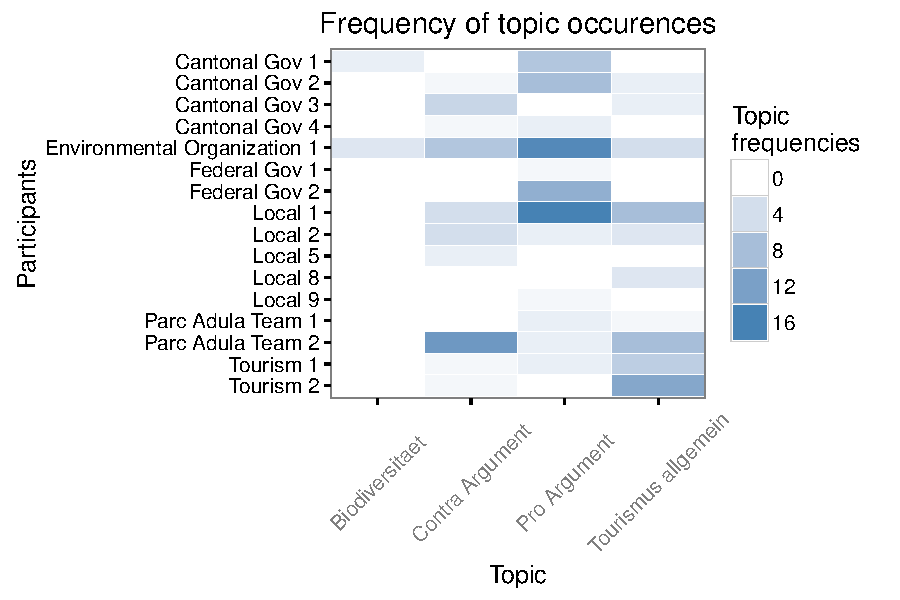
\includegraphics{publication_files/figure-latex/plotfreq-1.pdf}
\caption{Frequency matrix of a selected list of topics across the
various representants}
\end{figure}

\textbf{Notes on reproducibility:} Depending on the data to analize
privacy plays a role. While for the analysis itself the data is being
anonymised, storing the raw or preprocessed data on a public repository
may poses issues regarding the privacy of the data.

\subsubsection{Google query timeline}\label{google-query-timeline}

Overview on the Google trend evolution on the search query: \emph{Parc
Adula}
(\href{https://www.google.com/trends/explore?date=all\&q=parc\%20adula}{url},
provides a CSV file). The timeline shows overall a small amount of
queries for this word combination, with a spike on 2015-11-01. The has
been retrieved on August 11, 2016.

\textbf{Notes on reproducibility:} Due to license restrictions of the
open geodata it is not possible to store the data on a public Git
repository. The included script \texttt{R/loadMapData.r} downloads the
data directly from the link provided in the geodata catalog infobox of
\url{http://maps.geo.admin.ch}

\begin{figure}[htbp]
\centering
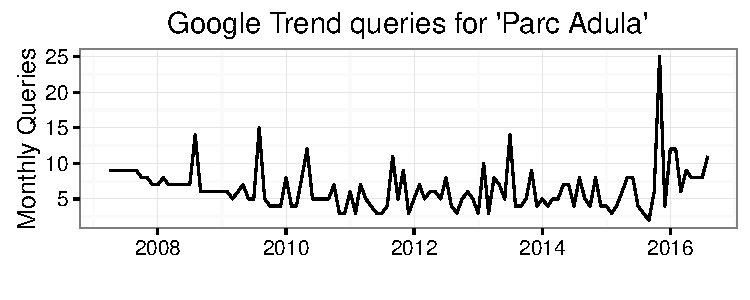
\includegraphics{publication_files/figure-latex/googleTrend-1.pdf}
\caption{Timeline of queries for Parc Adula set in the Google search
engine}
\end{figure}

\subsubsection{Case study area}\label{case-study-area}

Parc Adula is situated in Switzerland in the border region of the
cantons Ticino and Grisons. The map below presents the current outer
perimiter of the planned national parc.

\textbf{Notes on reproducibility:} Due to license restrictions of the
open geodata it is not possible to store the data on a public Git
repository. The included script \texttt{R/loadMapData.r} downloads the
data directly from the link provided in the geodata catalog infobox of
\url{http://maps.geo.admin.ch}

\begin{figure}
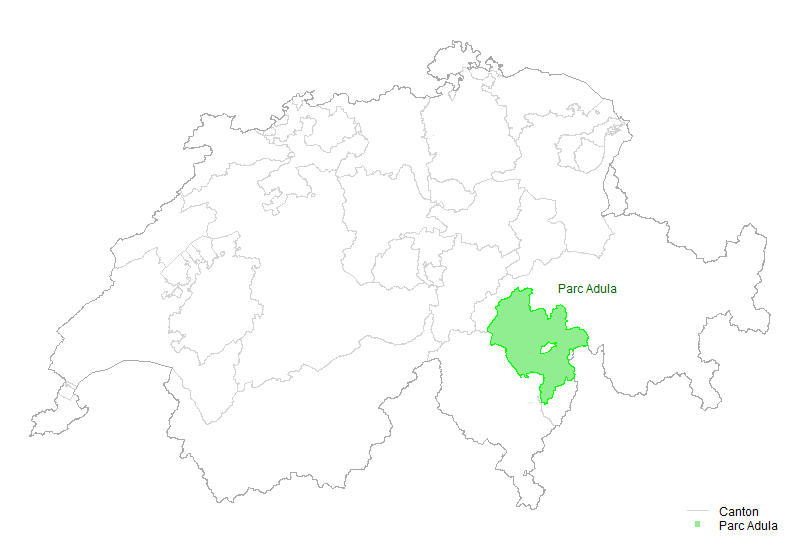
\includegraphics[width=0.6\linewidth]{figures/map} \caption{Planned perimeter of Parc Adula, Switzerland, Data source: Swisstopo}\label{fig:map}
\end{figure}

\subsection{Discussion \& Conclusions}\label{discussion-conclusions}

This template based on data of an ongoing presents some typical examples
maybe used in a publication writen in RMarkdown. It presents the
inclusion of data and analysis, features plots, tables, and various
markdown elements and shows how to integrate literature. The generated
files in \emph{PDF}, \emph{Word} or \emph{HTML} often still need fine
some fine-tuning afterwards (particularly in Latex). However, it still
presents a great way documenting the research process, that is easily
shareable and the generation of the initial drafts.

\section{Acknowledgements}\label{acknowledgements}

The Reproducible Research workshop was supported by the InnoPool of the
Department of Geography, University of Zurich.

\section*{References}\label{references}
\addcontentsline{toc}{section}{References}

\hypertarget{refs}{}
\hypertarget{ref-Baker2016}{}
Baker M, 2016, 1,500 scientists lift the lid on reproducibility.
\emph{Nature}. 533(7604):452--454.

\hypertarget{ref-Brunsdon2015}{}
Brunsdon C, 2015, Quantitative methods I: Reproducible research and
quantitative geography. Progress in Human Geography. doi:
\href{https://doi.org/10.1177/0309132515599625}{10.1177/0309132515599625}

\hypertarget{ref-Buckheit1995}{}
Buckheit J, Donoho D, 1995, WaveLab and Reproducible Research.
\emph{Wavelets and Statistics}. 10355--81.

\hypertarget{ref-Nature2016}{}
Editorial, 2016, Reality check on reproducibility. \emph{Nature}.
533(7604):437--437.

\hypertarget{ref-Healy2016}{}
Healy K, 2016, The Plain Person's Guide to Plain Text Social Science.
Healy2016

\hypertarget{ref-Healy2011}{}
Healy K, 2011, Choosing Your Workflow Applications. \emph{The Political
Methodologist}. 18(2):9--18.

\hypertarget{ref-Leveque2012}{}
LeVeque RJ, Mitchell IM, Stodden V, 2012, Reproducible research for
scientific computing: Tools and strategies for changing the culture.
\emph{Computing in Science \& Engineering}. 14(4):13--17.

\hypertarget{ref-Nuest2011}{}
Nüst D, Stasch C, Pebesma E, 2011, Connecting R to the sensor Web. In:
Lecture notes in geoinformation and cartography. 227--246

\hypertarget{ref-Pebesma2012}{}
Pebesma E, Nüst D, Bivand R, 2012, The R software environment in
reproducible geoscientific research. \emph{Eos, Transactions American
Geophysical Union}. 93(16):163--163.

\hypertarget{ref-Vandewalle2012}{}
Vandewalle P, 2012, Code Sharing Is Associated with Research Impact in
Image Processing. \emph{Computing in Science \& Engineering}.
14(4):42--47.

\end{document}
